%{{第十七回}}{第十七回}}

\chapter{大观园试才题对额\hspace{.5em}荣国府归省庆元宵}

{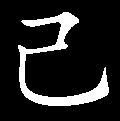
\includegraphics[width=3mm]{../Images/00003}\kaishu 此回宜分二回方妥。}

{\kaishu 宝玉系诸艳之冠,故大观园对额必得玉兄题跋,且暂题灯匾联上,再请赐题。此千妥万当之章法。}

诗曰:

豪华虽足羡,离别却难堪。博得虚名在,谁人识苦甘?{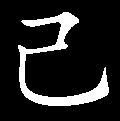
\includegraphics[width=3mm]{../Images/00003}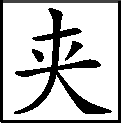
\includegraphics[width=3mm]{../Images/00012}\footnotesize \kaishu 好诗,全是讽刺。近之谚云:``又要马儿好,又要马儿不吃草。''真骂尽无厌贪痴之辈。}

话说秦钟既死,宝玉痛哭不已,李贵等好容易劝解半日方住,归时犹是凄恻哀痛。贾母帮了几十两银子,外又另备奠仪,宝玉去吊纸。七日后便送殡掩埋了,别无述记。只有宝玉日日思慕感悼,然亦无可如何了。{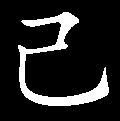
\includegraphics[width=3mm]{../Images/00003}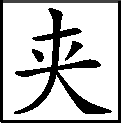
\includegraphics[width=3mm]{../Images/00012}\footnotesize \kaishu 每于此等文后便用此语作结,是板定大章法,亦是此书大旨。}

又不知历几何时,{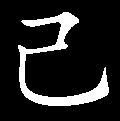
\includegraphics[width=3mm]{../Images/00003}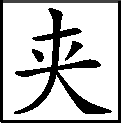
\includegraphics[width=3mm]{../Images/00012}\footnotesize \kaishu 年表如此写,亦妙! {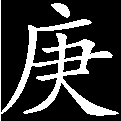
\includegraphics[width=3mm]{../Images/00004}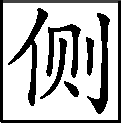
\includegraphics[width=3mm]{../Images/00011}\footnotesize \kaishu 惯用此等章法。}}这日贾珍等来回贾政:``园内工程俱已告竣,大老爷已瞧过了,只等老爷瞧了,或有不妥之处,再行改造,好题匾额对联的。''贾政听了,沉思一回,说道:``这匾额对联倒是一件难事。论理该请贵妃赐题才是,然贵妃若不亲睹其景,大约亦必不肯妄拟;若直待贵妃游幸过再请题,偌大景致,若干亭榭,无字标题,也觉寥落无趣,任有花柳山水,也断不能生色。''众清客在旁笑答道:``老世翁所见极是。如今我们有个愚见:各处匾额对联断不可少,亦断不可定名。如今且按其景致,或两字、三字、四字,虚合其意,拟了出来,暂且做出灯匾联悬了。待贵妃游幸时,再请定名,岂不两全?''贾政等听了,都道:``所见不差。我们今日且看看去,只管题了,若妥当便用;不妥时,然后将雨村请来,令他再拟。''{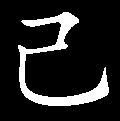
\includegraphics[width=3mm]{../Images/00003}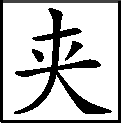
\includegraphics[width=3mm]{../Images/00012}\footnotesize \kaishu 点雨村,照应前文。}众人笑道:``老爷今日一拟定佳,何必又待雨村。''贾政笑道:``你们不知,我自幼于花鸟山水题咏上就平平;{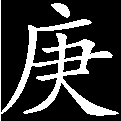
\includegraphics[width=3mm]{../Images/00004}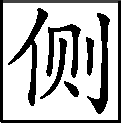
\includegraphics[width=3mm]{../Images/00011}\footnotesize \kaishu 是纱帽头口气。}如今上了年纪,且案牍劳烦,于这怡情悦性文章上更生疏了,纵拟了出来,不免迂腐古板,反不能使花柳园亭生色,似不妥协,反没意思。''{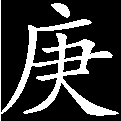
\includegraphics[width=3mm]{../Images/00004}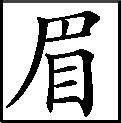
\includegraphics[width=3mm]{../Images/00010}\footnotesize \kaishu 政老情字如此写。壬午季春。畸笏。}众清客笑道:``这也无妨。我们大家看了公拟,各举其长,优则存之,劣则删之,未为不可。''贾政道:``此论极是。且喜今日天气和暖,大家去逛逛{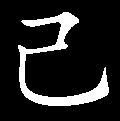
\includegraphics[width=3mm]{../Images/00003}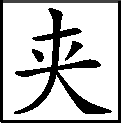
\includegraphics[width=3mm]{../Images/00012}\footnotesize \kaishu 音光,字去声,出《谐声字笺》。}。''说着起身,引众人前往。

贾珍先去园中知会众人。可巧近日宝玉因思念秦钟,忧戚不尽,贾母常命人带他到园中来戏耍。{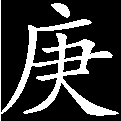
\includegraphics[width=3mm]{../Images/00004}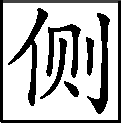
\includegraphics[width=3mm]{../Images/00011}\footnotesize \kaishu 现成榫楔,一丝不费力。若特唤出宝玉来,则成何文字?}此时亦才进去,忽见贾珍走来,向他笑道:``你还不出去,老爷就来了。''宝玉听了,带着奶娘小厮们,一溜烟就出园来。{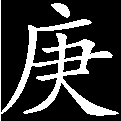
\includegraphics[width=3mm]{../Images/00004}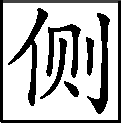
\includegraphics[width=3mm]{../Images/00011}\footnotesize \kaishu 不肖子弟来看形容。余初看之,不觉怒焉,盖谓作者形容余幼年往事,因思彼亦自写其照,何独余哉?信笔书之,供诸大众同一发笑。}方转过弯,顶头贾政引众客来了,躲之不及,只得一边站了。贾政近日因闻得塾掌称赞宝玉专能对对联,虽不喜读书,偏倒有些歪才情似的,{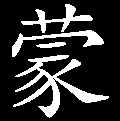
\includegraphics[width=3mm]{../Images/00006}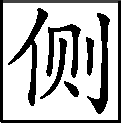
\includegraphics[width=3mm]{../Images/00011}\footnotesize \kaishu 如此顺笔写来,然却是宝玉正传。}今日偶然撞见这机会,便命他跟来。{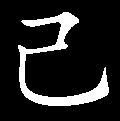
\includegraphics[width=3mm]{../Images/00003}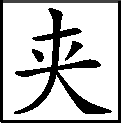
\includegraphics[width=3mm]{../Images/00012}\footnotesize \kaishu 如此偶然方妙,若特特唤来题额,真不成文矣。}宝玉只得随往,尚不知何意。

贾政刚至园门前,只见贾珍带领许多执事人来,一旁侍立。贾政道:``你且把园门都关上,我们先瞧了外面再进去。''{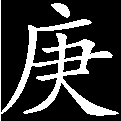
\includegraphics[width=3mm]{../Images/00004}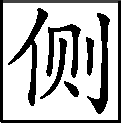
\includegraphics[width=3mm]{../Images/00011}\footnotesize \kaishu 是行家看法。}贾珍听说,命人将门关了。贾政先秉正看门。只见正门五间,上面桶瓦泥鳅脊;那门栏窗槅,皆是细雕新鲜花样,并无朱粉涂饰;一色水磨群墙,{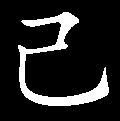
\includegraphics[width=3mm]{../Images/00003}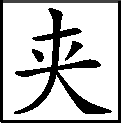
\includegraphics[width=3mm]{../Images/00012}\footnotesize \kaishu 门雅,墙雅,不落俗套。}下面白石台矶,凿成西番草花样。左右一望,皆雪白粉墙,下面虎皮石,随势砌去,果然不落富丽俗套,自是欢喜。遂命开门,只见迎门一带翠嶂挡在前面。{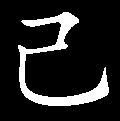
\includegraphics[width=3mm]{../Images/00003}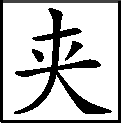
\includegraphics[width=3mm]{../Images/00012}\footnotesize \kaishu 掩隐的好。}众清客都道:``好山,好山!''贾政道:``非此一山,一进来园中所有之景悉入目中,则有何趣。''众人道:``极是。非胸中大有邱壑,焉想及此。''说毕,往前一望,见白石崚嶒,{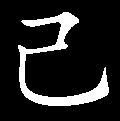
\includegraphics[width=3mm]{../Images/00003}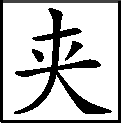
\includegraphics[width=3mm]{../Images/00012}\footnotesize \kaishu 想入其中,一时难辩方向。用``前''``后''``这边''``那边''等字,正是不辨东西。}或如鬼怪,或如猛兽,纵横拱立,上面苔藓成斑,藤萝掩映,{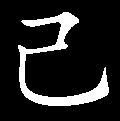
\includegraphics[width=3mm]{../Images/00003}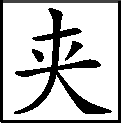
\includegraphics[width=3mm]{../Images/00012}\footnotesize \kaishu 曾用两处旧有之园所改,故如此写方可,细极。}其中微露羊肠小径,{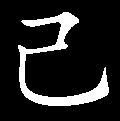
\includegraphics[width=3mm]{../Images/00003}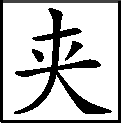
\includegraphics[width=3mm]{../Images/00012}\footnotesize \kaishu 好景界,山子野精于此技。◇此是小径,非行车辇道,今贾政原欲游览其景,故将此等处写之。想其通路大道,自是堂堂冠冕气象,无庸细写者也。后于省亲之时已得知矣。}贾政道:``我们就从此小径游去,回来由那一边出去,方可遍览。''

说毕,命贾珍在前引导,自己扶了宝玉,逶迤进入山口。{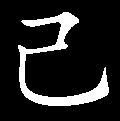
\includegraphics[width=3mm]{../Images/00003}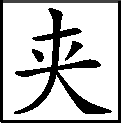
\includegraphics[width=3mm]{../Images/00012}\footnotesize \kaishu 此回乃一部之纲绪,不得不细写,尤不可不细批注。盖后文十二钗书,出入来往之境,方不能错乱,观者亦如身临足到矣。今贾政虽进的是正门,却行的是僻路,按此一大园,羊肠鸟道不止几百十条,穿东度西,临山过水,万勿以今日贾政所行之径,考其方向基址。故正殿反于末后写之,足见未由大道而往,乃逶迤转折而经也。 {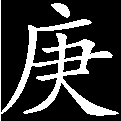
\includegraphics[width=3mm]{../Images/00004}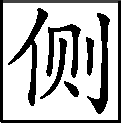
\includegraphics[width=3mm]{../Images/00011}\footnotesize \kaishu 宝玉此刻已料定吉多凶少。}}抬头忽见山上有镜面白石一块,{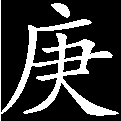
\includegraphics[width=3mm]{../Images/00004}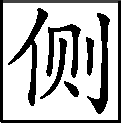
\includegraphics[width=3mm]{../Images/00011}\footnotesize \kaishu 新奇。}正是迎面留题处。{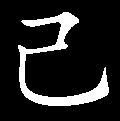
\includegraphics[width=3mm]{../Images/00003}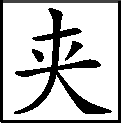
\includegraphics[width=3mm]{../Images/00012}\footnotesize \kaishu 留题处便精,不必限定凿金镂银一色恶俗,赖及枣梨之力。}贾政回头笑道:``诸公请看,此处题以何名方妙?''众人听说,也有说该题``叠翠''二字,也有说该题``锦嶂''的,又有说``赛香炉''的,又有说``小终南''的,种种名色,不止几十个。原来众客心中早知贾政要试宝玉的功业进益何如,只将些俗套来敷衍。宝玉亦料定此意。{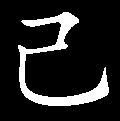
\includegraphics[width=3mm]{../Images/00003}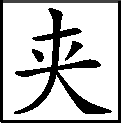
\includegraphics[width=3mm]{../Images/00012}\footnotesize \kaishu 补明好。}贾政听了,便回头命宝玉拟来。宝玉道:``尝闻古人有云:`编新不如述旧,刻古终胜雕今。'{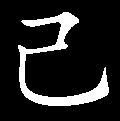
\includegraphics[width=3mm]{../Images/00003}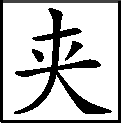
\includegraphics[width=3mm]{../Images/00012}\footnotesize \kaishu 未闻古人说此两句,却又似有者。}况此处并非主山正景,原无可题之处,不过是探景一进步耳。{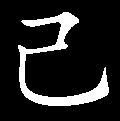
\includegraphics[width=3mm]{../Images/00003}\includegraphics[width=3mm]{../Images/00012}\footnotesize \kaishu 此论却是。}莫如直书`曲径通幽处'这句旧诗在上,倒还大方气派。''众人听了,都赞道:``是极!二世兄天分高,才情远,不似我们读腐了书的。''贾政笑道:``不当谬奖。他年小,不过以一知充十用,取笑罢了。再俟选拟。''

说着,进入石洞来,只见佳木茏葱,奇花熌灼,一带清流,从花木深处曲折泻于石隙之下。{\includegraphics[width=3mm]{../Images/00003}\includegraphics[width=3mm]{../Images/00012}\footnotesize \kaishu 这水是人力引来做的。}再进数步,渐向北边,{\includegraphics[width=3mm]{../Images/00003}\includegraphics[width=3mm]{../Images/00012}\footnotesize \kaishu 细极。后文所以云进贾母卧房后之角门,是诸钗日相来往之境也。后文又云,诸钗所居之处,只在西北一带,最近贾母卧室之后,皆从此``北''字而来。}平坦宽豁,两边飞楼插空,雕甍绣槛,皆隐于山坳树杪之间。俯而视之,则清溪泻雪,石磴穿云,{\includegraphics[width=3mm]{../Images/00003}\includegraphics[width=3mm]{../Images/00012}\footnotesize \kaishu 前已写山至宽处,此则由低处至高处,各景皆遍。}白石为栏,环抱池沿,石桥三港,兽面衔吐。桥上有亭。{\includegraphics[width=3mm]{../Images/00003}\includegraphics[width=3mm]{../Images/00012}\footnotesize \kaishu 前已写山写石,今则写池写楼,各景皆遍。}贾政与诸人上了亭子,倚栏坐了,{\includegraphics[width=3mm]{../Images/00003}\includegraphics[width=3mm]{../Images/00012}\footnotesize \kaishu 此亭大抵四通八达,为诸小径之咽喉要路。}因问:``诸公以何题此?''诸人都道:``当日欧阳公《醉翁亭记》有云:`有亭翼然。'就名`翼然'。''贾政笑道:``\,`翼然'虽佳,但此亭压水而成,还须偏于水题方称。依我拙裁,欧阳公之`泻出于两峰之间',竟用他这一个`泻'字。''有一客道:``是极,是极。竟是`泻玉'二字妙。''贾政拈髯寻思,因抬头见宝玉侍侧,便笑命他也拟一个来。宝玉听说,连忙回道:``老爷方才所议已是。但是如今追究了去,似乎当日欧阳公题酿泉用一`泻'字则妥,今日此泉若亦用`泻'字,则觉不妥。况此处虽为省亲驻跸别墅,亦当入于应制之例,用此等字眼,亦觉粗陋不雅。求再拟较此蕴藉含蓄者。''贾政笑道:``诸公听此论若如?方才众人编新,你又说不如述古;如今我们述古,你又说粗陋不妥。你且说你的来我听。''宝玉道:``有用`泻玉'二字,则莫若`沁芳'{\includegraphics[width=3mm]{../Images/00004}\includegraphics[width=3mm]{../Images/00011}\footnotesize \kaishu 真新雅。}二字,{\includegraphics[width=3mm]{../Images/00003}\includegraphics[width=3mm]{../Images/00012}\footnotesize \kaishu 果然。}岂不新雅?''贾政拈髯点头不语。{\includegraphics[width=3mm]{../Images/00004}\includegraphics[width=3mm]{../Images/00010}\footnotesize \kaishu 六字是严父大露悦容也。壬午春。}众人都忙迎合,赞宝玉才情不凡。贾政道:``匾上二字容易,再作一副七言对联来。''宝玉听说,立于亭上,四顾一望,便机上心来,乃念道:

绕堤柳借三篙翠,{\includegraphics[width=3mm]{../Images/00003}\includegraphics[width=3mm]{../Images/00012}\footnotesize \kaishu 要紧,贴切水字。}

隔岸花分一脉香。{\includegraphics[width=3mm]{../Images/00003}\includegraphics[width=3mm]{../Images/00012}\footnotesize \kaishu 恰极,工极!绮靡秀媚,香奁正体。}

贾政听了,点头微笑。众人先称赞不已。

于是出亭过池,一山一石,一花一木,莫不着意观览。{\includegraphics[width=3mm]{../Images/00003}\includegraphics[width=3mm]{../Images/00012}\footnotesize \kaishu 浑写两句,已见经行处愈远,更至北一路矣。}忽抬头看见前面一带粉垣,里面数楹修舍,有千百竿翠竹遮映。众人都道:``好个所在!''{\includegraphics[width=3mm]{../Images/00004}\includegraphics[width=3mm]{../Images/00011}\footnotesize \kaishu 此方可为颦儿之居。}于是大家进入,只见入门便是曲折游廊,{\includegraphics[width=3mm]{../Images/00003}\includegraphics[width=3mm]{../Images/00012}\footnotesize \kaishu 不犯超手游廊。}阶下石子漫成甬路。上面小小两三间房舍,一明两暗,里面都是合着地步打就的床几椅案。从里间房内又得一小门,出去则是后院,有大茉莉花兼着芭蕉。又有两间小小退步。后院墙下忽开一隙,得泉一派,开沟仅尺许,灌入墙内,绕阶缘屋至前院,盘旋竹下而出。

贾政笑道:``这一处{\includegraphics[width=3mm]{../Images/00004}\includegraphics[width=3mm]{../Images/00011}\footnotesize \kaishu 一处。}还罢了。若能月夜坐此窗下读书,不枉虚生一世。''说毕,看着宝玉,唬的宝玉忙垂了头。{\includegraphics[width=3mm]{../Images/00003}\includegraphics[width=3mm]{../Images/00012}\footnotesize \kaishu 点一笔。}众客忙用话开释,{\includegraphics[width=3mm]{../Images/00003}\includegraphics[width=3mm]{../Images/00012}\footnotesize \kaishu 客不可不有。}又说道:``此处的匾该题四个字。''贾政笑问:``那四字?''一个道是``淇水遗风。''贾政道:``俗。''{\includegraphics[width=3mm]{../Images/00003}\includegraphics[width=3mm]{../Images/00012}\footnotesize \kaishu 余亦如此。}又一个是``睢园雅迹''。贾政道:``也俗。''贾珍笑道:``还是宝兄弟拟一个来。''{\includegraphics[width=3mm]{../Images/00004}\includegraphics[width=3mm]{../Images/00010}\footnotesize \kaishu 又换一章法。壬午春。}贾政道:``他未曾作,先要议论人家的好歹,可见就是个轻薄人。''{\includegraphics[width=3mm]{../Images/00004}\includegraphics[width=3mm]{../Images/00011}\footnotesize \kaishu 知子者莫如父。}众客道:``议论的极是,其奈他何。''贾政忙道:``休如此纵了他。''因命他道:``今日任你狂为乱道,先设议论来,然后方许你作。{\includegraphics[width=3mm]{../Images/00003}\includegraphics[width=3mm]{../Images/00012}\footnotesize \kaishu 又一格式,不然,不独死板,且亦大失严父素体。 {\includegraphics[width=3mm]{../Images/00004}\includegraphics[width=3mm]{../Images/00010}\footnotesize \kaishu 于作诗文时,虽政老亦有如此令旨,可知严父亦无可奈何也。不学纨绔来看。畸笏。}}方才众人说的,可有使得的?''宝玉见问,答道:``都似不妥。''{\includegraphics[width=3mm]{../Images/00003}\includegraphics[width=3mm]{../Images/00012}\footnotesize \kaishu 明知是故意要他搬驳议论,落得肆行施展。}贾政冷笑道:``怎么不妥?''宝玉道:``这是第一处行幸之处,必须颂圣方可。若用四字的匾,又有古人现成的,何必再作。''贾政道:``难道`淇水'`睢园'不是古人的?''宝玉道:``这太板腐了。莫若`有凤来仪'四字。''{\includegraphics[width=3mm]{../Images/00003}\includegraphics[width=3mm]{../Images/00012}\footnotesize \kaishu 果然,妙在双关暗合。}众人都哄然叫妙。贾政点头道:``畜生,畜生,可谓`管窥蠡测'矣。''因命:``再题一联来。''宝玉便念道:

宝鼎茶闲烟尚绿,{\includegraphics[width=3mm]{../Images/00003}\includegraphics[width=3mm]{../Images/00012}\footnotesize \kaishu ``尚''字妙极!不必说竹,然恰恰是竹中精舍。}

幽窗棋罢指犹凉。{\includegraphics[width=3mm]{../Images/00003}\includegraphics[width=3mm]{../Images/00012}\footnotesize \kaishu ``犹''字妙!``尚绿''、``犹凉''四字,便如置身于森森万竿之中。}

贾政摇头说道:``也未见长。''说毕,引众人出来。

方欲走时,忽又想起一事来,{\includegraphics[width=3mm]{../Images/00003}\includegraphics[width=3mm]{../Images/00011}\footnotesize \kaishu 不板。}因问贾珍道:``这些院落房宇并几案桌椅都算有了,{\includegraphics[width=3mm]{../Images/00004}\includegraphics[width=3mm]{../Images/00011}\footnotesize \kaishu 此一顿少不得。}还有那些帐幔帘子并陈设玩器古董,可也都是一处一处合式配就的?''{\includegraphics[width=3mm]{../Images/00003}\includegraphics[width=3mm]{../Images/00012}\footnotesize \kaishu 大篇长文,不如此顿,则成何话说?}贾珍回道:``那陈设的东西早已添了许多,自然临期合式陈设。帐幔帘子,昨日听见琏兄弟说,还不全。那原是一起工程之时就画了各处的图样,量准尺寸,就打发人办去的。想必昨日得了一半。''{\includegraphics[width=3mm]{../Images/00003}\includegraphics[width=3mm]{../Images/00012}\footnotesize \kaishu 补出近日忙冗,千头万绪景况。}贾政听了,便知此事不是贾珍的首尾,便令人去唤贾琏。

一时贾琏赶来。{\includegraphics[width=3mm]{../Images/00003}\includegraphics[width=3mm]{../Images/00012}\footnotesize \kaishu 写出忙冗景况。}贾政问他共有几种,现今得了几种,尚欠几种。贾琏见问,忙向靴桶内取靴掖内装的一个纸折略节来,{\includegraphics[width=3mm]{../Images/00003}\includegraphics[width=3mm]{../Images/00012}\footnotesize \kaishu 细极!从头至尾,誓不作一笔安逸苟且之笔。}看了一看,回道:``妆{\includegraphics[width=3mm]{../Images/00003}\includegraphics[width=3mm]{../Images/00012}\footnotesize \kaishu 一字一句。}、蟒、绣、堆,刻丝、弹墨{\includegraphics[width=3mm]{../Images/00003}\includegraphics[width=3mm]{../Images/00012}\footnotesize \kaishu 二字一句。},并各色绸绫大小幔子一百二十架,昨日得了八十架,下欠四十架。帘子二百挂,昨日俱得了。外有猩猩毡帘二百挂,\href{../Text/part0021_split_000.html\#lnkback_2_a}{\textsuperscript{②}}金丝藤红漆竹帘二百挂,墨漆竹帘二百挂,五彩线络盘花帘二百挂,每样得了一半,也不过秋天都全了。椅搭、桌围、床裙、桌套,每分一千二百件,也有了。''

一面走,一面说,{\includegraphics[width=3mm]{../Images/00003}\includegraphics[width=3mm]{../Images/00012}\footnotesize \kaishu 是极!}倏尔青山斜阻。{\includegraphics[width=3mm]{../Images/00003}\includegraphics[width=3mm]{../Images/00012}\footnotesize \kaishu ``斜''字细,不必拘定方向。诸钗所居之处,若稻香村、潇湘馆、怡红院、秋爽斋、蘅芜苑等,都相隔不远,究竟只在一隅。然处置得巧妙,使人见其千邱万壑,恍然不知所穷,所谓会心处不在乎远。大抵一山一水,一木一石,全在人之穿插布置耳。}转过山怀中,隐隐露出一带黄泥筑就矮墙,墙头上皆用稻茎掩护。{\includegraphics[width=3mm]{../Images/00003}\includegraphics[width=3mm]{../Images/00012}\footnotesize \kaishu 配的好!}有几百株杏花,如喷火蒸霞一般。里面数楹茅屋。外面却是桑、榆、槿、柘,各色树稚新条,随其曲折,编就两溜青篱。篱外山坡之下,有一土井,旁有桔槔辘轳之属。下面分畦列亩,佳蔬菜花,漫然无际。{\includegraphics[width=3mm]{../Images/00003}\includegraphics[width=3mm]{../Images/00012}\footnotesize \kaishu 阅至此,又笑别部小说中,一万个花园中,皆是牡丹亭、芍药圃、雕栏画栋、琼榭朱楼,略不见差别。}

贾政笑道:``倒是此处有些道理。固然系人力穿凿,此时一见,未免勾引起我归农之意。{\includegraphics[width=3mm]{../Images/00003}\includegraphics[width=3mm]{../Images/00012}\footnotesize \kaishu 极热中偏以冷笔点之,所以为妙。}我们且进去歇息歇息。''说毕,方欲进篱门去,忽见路旁有一石碣,亦为留题之备。{\includegraphics[width=3mm]{../Images/00003}\includegraphics[width=3mm]{../Images/00012}\footnotesize \kaishu 更恰当。若有悬额之处,或再用镜面石,岂复成文哉?忽想到``石碣''二字,又托出许多郊野气色来,一肚皮千邱万壑,只在这石碣上。 {\includegraphics[width=3mm]{../Images/00004}\includegraphics[width=3mm]{../Images/00011}\footnotesize \kaishu 真妙真新。}}众人笑道:``更妙,更妙!此处若悬匾待题,则田舍家风一洗尽矣。立此一碣,又觉生色许多,非范石湖田家之咏不足以尽其妙。''{\includegraphics[width=3mm]{../Images/00003}\includegraphics[width=3mm]{../Images/00012}\footnotesize \kaishu 客不可不养。 {\includegraphics[width=3mm]{../Images/00004}\includegraphics[width=3mm]{../Images/00011}\footnotesize \kaishu 赞得是,这个篾翁有些意思。}}贾政道:``诸公请题。''众人道:``方才世兄有云,`编新不如述旧',此处古人已道尽矣,莫若直书`杏花村'妙极。''贾政听了,笑向贾珍道:``正亏提醒了我。此处都妙极,只是还少一个酒幌,明日竟作一个,不必华丽,就依外面村庄的式样作来,用竹竿挑在树梢。''贾珍答应了,又回道:``此处竟还不可养别的雀鸟,只是买些鹅鸭鸡类,才都相称了。''贾政与众人都道:``更妙。''贾政又向众人道:```杏花村'固佳,只是犯了正名,村名直待请名方可。''众客都道:``是呀。如今虚的,便是什么字样好?''大家想着,宝玉却等不得了,{\includegraphics[width=3mm]{../Images/00003}\includegraphics[width=3mm]{../Images/00012}\footnotesize \kaishu 又换一格方不板。}也不等贾政的命,{\includegraphics[width=3mm]{../Images/00003}\includegraphics[width=3mm]{../Images/00012}\footnotesize \kaishu 忘情有趣。}便说道:``旧诗有云:`红杏梢头挂酒旗。'如今莫若`杏帘在望'{\includegraphics[width=3mm]{../Images/00003}\includegraphics[width=3mm]{../Images/00012}\footnotesize \kaishu 妙在一``在''字。}四字。''众人都道:``好个`在望'!又暗合`杏花村'意。''宝玉冷笑道:{\includegraphics[width=3mm]{../Images/00003}\includegraphics[width=3mm]{../Images/00012}\footnotesize \kaishu 忘情最妙。}``村名若用`杏花'二字,则俗陋不堪了。又有古人诗云:`柴门临水稻花香。'何不就用`稻香村'的妙?''众人听了,亦发哄声拍手道:``妙!''贾政一声喝断:``无知的业障!{\includegraphics[width=3mm]{../Images/00004}\includegraphics[width=3mm]{../Images/00010}\footnotesize \kaishu 爱之至,喜之至,故作此语。◇作者至此,宁不笑杀?壬午春。}你能知道几个古人,能记得几首熟诗,也敢在老先生前卖弄!你方才那些胡说的,不过是试你的清浊,取笑而已,你就认真了!''说着,引众人步入茆堂,里面纸窗木榻,富贵气象一洗皆尽。贾政心中自是喜欢,却瞅宝玉道:``此处如何?''众人见问,都忙悄悄的推宝玉,教他说好。宝玉不听人言,便应声道:``不及`有凤来仪'多矣。''{\includegraphics[width=3mm]{../Images/00003}\includegraphics[width=3mm]{../Images/00012}\footnotesize \kaishu 公然自定名,妙!}贾政听了道:``无知的蠢物!你只知朱楼画栋,恶赖富丽为佳,那里知道这清幽气象。终是不读书之过!''宝玉忙答道:``老爷教训的固是,但古人常云`天然'二字,不知何意?''

众人见宝玉牛心,都怪他呆痴不改。今见问``天然''二字,众人忙道:``别的都明白,为何连`天然'不知?`天然'者,天之自然而有,非人力之所成也。''宝玉道:``却又来!此处置一田庄,分明见得人力穿凿扭捏而成。远无邻村,近不负郭,背山山无脉,临水水无源,高无隐寺之塔,下无通市之桥,峭然孤出,似非大观。争似先处有自然之理,得自然之气,虽种竹引泉,亦不伤于穿凿。古人云`天然图画'四字,正畏非其地而强为其地,非其山而强为其山,虽百般精而终不相宜\ldots{}\ldots{}''未及说完,贾政气的喝命:``叉出去!''刚出去,又喝命:``回来!''命再题一联:``若不通,一并打嘴!''{\includegraphics[width=3mm]{../Images/00004}\includegraphics[width=3mm]{../Images/00010}\footnotesize \kaishu 所谓``奈何他不得''也,呵呵!畸笏。}宝玉只得念道:

新涨绿添浣葛处,{\includegraphics[width=3mm]{../Images/00004}\includegraphics[width=3mm]{../Images/00012}\footnotesize \kaishu 采《诗》颂圣最恰当。}

好云香护采芹人。{\includegraphics[width=3mm]{../Images/00004}\includegraphics[width=3mm]{../Images/00012}\footnotesize \kaishu 采《风》采《雅》都恰当。然冠冕中又不失香奁格调。}

贾政听了,摇头说:``更不好。''一面引人出来,转过山坡,穿花度柳,抚石依泉,过了荼蘼架,再入木香棚,越牡丹亭,度芍药圃,入蔷薇院,出芭蕉坞,盘旋曲折。{\includegraphics[width=3mm]{../Images/00003}\includegraphics[width=3mm]{../Images/00012}\footnotesize \kaishu 略用套语一束,与前顿破格不板。}忽闻水声潺湲,泻出石洞,上则萝薜倒垂,下则落花浮荡。{\includegraphics[width=3mm]{../Images/00003}\includegraphics[width=3mm]{../Images/00012}\footnotesize \kaishu 仍是沁芳溪矣,究竟基址不大,全是曲折掩隐之巧可知。}众人都道:``好景,好景!''贾政道:``诸公题以何名?''众人道:``再不必拟了,恰恰乎是`武陵源'三个字。''贾政笑道:``又落实了,而且陈旧。''众人笑道:``不然就用`秦人旧舍'四字也罢了。''宝玉道:``这越发过露了。`秦人旧舍'说避乱之意,如何使得?莫若`蓼汀花溆'四字。''贾政听了,更批胡说。

于是要进港洞时,又想起有船无船。贾珍道:``采莲船共四只,座船一只,如今尚未造成。''贾政笑道:``可惜不得入了。''贾珍道:``从山上盘道亦可进去。''说毕,在前导引,大家攀藤抚树过去。只见水上落花愈多,其水愈清,溶溶荡荡,曲折萦纡。池边两行垂柳,杂着桃杏,遮天蔽日,真无一些尘土。忽见柳阴中又露出一个折带朱栏板桥来,{\includegraphics[width=3mm]{../Images/00003}\includegraphics[width=3mm]{../Images/00012}\footnotesize \kaishu 此处才见一朱粉字样。绿柳红桥,此等点缀亦不可少。后文写芦雪广则曰蜂腰板桥,都施之得宜,非一幅死稿也。}度过桥去,诸路可通,{\includegraphics[width=3mm]{../Images/00003}\includegraphics[width=3mm]{../Images/00012}\footnotesize \kaishu 补四字,细极!不然后文宝钗来往,则将日日爬山越岭矣。记清此处,则知后文宝玉所行常径,非此处也。}便见一所清凉瓦舍,一色水磨砖墙,清瓦花堵。那大主山所分之脉,{\includegraphics[width=3mm]{../Images/00003}\includegraphics[width=3mm]{../Images/00012}\footnotesize \kaishu 两见大主山,稻香村又云怀中,不写主山,而主山处处映带连络不断可知矣。}皆穿墙而过。{\includegraphics[width=3mm]{../Images/00003}\includegraphics[width=3mm]{../Images/00012}\footnotesize \kaishu 好想。}

贾政道:``此处这所房子,无味的很。''{\includegraphics[width=3mm]{../Images/00003}\includegraphics[width=3mm]{../Images/00012}\footnotesize \kaishu 先故顿此一笔,使后文愈觉生色,未扬先抑之法。盖钗、颦对峙有甚难写者。}因而步入门时,忽迎面突出插天的大玲珑山石来,四面群绕各式石块,竟把里面所有房屋悉皆遮住,而且一株花木也无。{\includegraphics[width=3mm]{../Images/00003}\includegraphics[width=3mm]{../Images/00012}\footnotesize \kaishu 更奇妙!}只见许多异草:或有牵藤的,或有引蔓的,或垂山巅,或穿石隙,甚至垂檐绕柱,萦砌盘阶,{\includegraphics[width=3mm]{../Images/00003}\includegraphics[width=3mm]{../Images/00012}\footnotesize \kaishu 更妙!}或如翠带飘摇,或如金绳盘屈,或实若丹砂,或花如金桂,味芬气馥,非花香之可比。{\includegraphics[width=3mm]{../Images/00003}\includegraphics[width=3mm]{../Images/00012}\footnotesize \kaishu 前三处皆还在人意之中,此一处则今古书中未见之工程也。连用几``或''字,是从昌黎《南山诗》中学得。}贾政不禁道:``有趣!{\includegraphics[width=3mm]{../Images/00003}\includegraphics[width=3mm]{../Images/00012}\footnotesize \kaishu 前有``无味''二字,及云``有趣''二字,更觉生色,更觉重大。}只是不大认识。''有的说:``是薜荔藤萝。''贾政道:``薜荔藤萝不得如此异香。''宝玉道:``果然不是。这些之中也有藤萝薜荔,那香的是杜若蘅芜,那一种大约是茝兰,这一种大约是清葛,那一种是金?草,这一种是玉蕗藤,红的自然是紫芸,绿的定是青芷。{{\includegraphics[width=3mm]{../Images/00003}\includegraphics[width=3mm]{../Images/00012}\footnotesize \kaishu 金}?{草,见《字汇》。玉}蕗{,见《楚辞》``}菎蕗{杂于}黀{蒸''。}茝{、葛、芸、芷,皆不必注,见者太多。此书中异物太多,有人生之未闻未见者,然实系所有之物,或名差理同者亦有之。}}想来《离骚》《文选》等书上所有的那些异草,也有叫作什么藿蒳姜荨\href{../Text/part0021_split_000.html\#lnkback_3_a}{\textsuperscript{③}}的,也有叫什么纶组紫绛的,还有石帆、水松、扶留等样,{\includegraphics[width=3mm]{../Images/00003}\includegraphics[width=3mm]{../Images/00012}\footnotesize \kaishu 左太冲《吴都赋》。}又有叫什么绿荑的,还有什么丹椒、蘼芜、风连。{\includegraphics[width=3mm]{../Images/00003}\includegraphics[width=3mm]{../Images/00012}\footnotesize \kaishu 以上《蜀都赋》。}如今年深岁改,人不能识,故皆像形夺名,渐渐的唤差了,也是有的。''{\includegraphics[width=3mm]{../Images/00003}\includegraphics[width=3mm]{../Images/00012}\footnotesize \kaishu 自实注一笔,妙!}未及说完,贾政喝道:``谁问你来!''{\includegraphics[width=3mm]{../Images/00003}\includegraphics[width=3mm]{../Images/00012}\footnotesize \kaishu 又一样止法。}唬的宝玉倒退,不敢再说。

贾政因见两边俱是超手游廊,便顺着游廊步入。只见上面五间清厦连着卷棚,四面出廊,绿窗油壁,更比前几处清雅不同。贾政叹道:``此轩中煮茶操琴,亦不必再焚名香矣。{\includegraphics[width=3mm]{../Images/00003}\includegraphics[width=3mm]{../Images/00012}\footnotesize \kaishu 前二处,一曰``月下读书'',一曰``勾引起归农之意'',此则``操琴煮茶'',断语皆妙。}此造已出意外,诸公必有佳作新题以颜其额,方不负此。''众人笑道:``再莫若`兰风蕙露'贴切了。''贾政道:``也只好用这四字。其联若何?''一人道:``我倒想了一对,大家批削改正。''念道是:

麝兰芳霭斜阳院,

杜若香飘明月洲。

众人道:``妙则妙矣,只是`斜阳'二字不妥。''那人道:``古人诗云:`蘼芜满手泣斜晖'。''众人道:``颓丧,颓丧。''又一人道:``我也有一联,诸公评阅评阅。''因念道:

三径香风飘玉蕙,

一庭明月照金兰。{\includegraphics[width=3mm]{../Images/00003}\includegraphics[width=3mm]{../Images/00012}\footnotesize \kaishu 此二联皆不过为钓宝玉之饵,不必认真批评。}

贾政拈髯沉吟,意欲也题一联。忽抬头见宝玉在旁不敢则声,因喝道:``怎么你应说话时又不说了?还要等人请教你不成!''宝玉听说,便回道:``此处并没有什么`兰麝'、`明月'、`洲渚'之类,若要这样着迹说来,就题二百联也不能完。''贾政道:``谁按着你的头,叫你必定说这些字样呢?''宝玉道:``如此说,匾上则莫若`蘅芷清芬'四字。对联则是:

吟成豆蔻才犹艳,

睡足酴醿梦也香。''{\includegraphics[width=3mm]{../Images/00003}\includegraphics[width=3mm]{../Images/00012}\footnotesize \kaishu 实佳。}

贾政笑道:``这是套的`书成蕉叶文犹绿',不足为奇。''众客道:``李太白`凤凰台'之作,全套`黄鹤楼',{\includegraphics[width=3mm]{../Images/00004}\includegraphics[width=3mm]{../Images/00011}\footnotesize \kaishu 这一位篾翁更有意思。}只要套得妙。如今细评起来,方才这一联,竟比`书成蕉叶'尤觉幽娴活泼。视`书成'之句,竟似套此而来。''贾政笑说:``岂有此理!''

说着,大家出来。行不多远,则见崇阁巍峨,层楼高起,面面琳宫合抱,迢迢复道萦纡,青松拂檐,玉栏绕砌,金辉兽面,彩焕螭头。贾政道:``这是正殿了。{\includegraphics[width=3mm]{../Images/00003}\includegraphics[width=3mm]{../Images/00012}\footnotesize \kaishu 想来此殿在园之正中。按园不是殿方之基,西北一带通贾母卧室后,可知西北一带是多宽出一带来的,诸钗始便于行也。}只是太富丽了些。''众人都道:``要如此方是。虽然贵妃崇节尚俭,天性恶繁悦朴,{\includegraphics[width=3mm]{../Images/00004}\includegraphics[width=3mm]{../Images/00011}\footnotesize \kaishu 写出贾妃身分天性。}然今日之尊,礼仪如此,不为过也。''一面说,一面走,只见正面{\includegraphics[width=3mm]{../Images/00003}\includegraphics[width=3mm]{../Images/00012}\footnotesize \kaishu 正面,细。}现出一座玉石牌坊来,上面龙蟠螭护,玲珑凿就。贾政道:``此处书以何文?''众人道:``必是`蓬莱仙境'方妙。''贾政摇头不语。宝玉见了这个所在,心中忽有所动,寻思起来,{\includegraphics[width=3mm]{../Images/00004}\includegraphics[width=3mm]{../Images/00010}\footnotesize \kaishu 一路顺顺逆逆,已成千邱万壑之景,若不有此一段大江截住,直成一盆景矣。作者从何落笔着想!}倒像那里曾见过的一般,却一时想不起那年月日的事了。{\includegraphics[width=3mm]{../Images/00003}\includegraphics[width=3mm]{../Images/00012}\footnotesize \kaishu 仍归于葫芦一梦之太虚玄境。}贾政又命他作题,宝玉只顾细思前景,全无心于此了。众人不知其意,只当他受了这半日的折磨,精神耗散,才尽辞穷了;再要考难逼迫,着了急,或生出事来,倒不便。遂忙都劝贾政:``罢,罢,明日再题罢了。''贾政心中也怕贾母不放心,{\includegraphics[width=3mm]{../Images/00003}\includegraphics[width=3mm]{../Images/00012}\footnotesize \kaishu 一笔不漏。}遂冷笑道:``你这畜生,也竟有不能之时了。也罢,限你一日,明日若再不能,我定不饶。这是要紧之处,更要好生作来!''

说着,引人出来,再一观望,原来自进门起,所行至此,才游了十之五六。{\includegraphics[width=3mm]{../Images/00003}\includegraphics[width=3mm]{../Images/00012}\footnotesize \kaishu 总住,妙!伏下后文所补等处。若都入此回写完,不独太繁,使后文冷落,亦且非《石头记》之笔。}又值人来回,有雨村处遣人来回话。{\includegraphics[width=3mm]{../Images/00003}\includegraphics[width=3mm]{../Images/00012}\footnotesize \kaishu 又一紧收,不能终局也。此处渐渐写雨村亲切,正为后文地步。伏脉千里,横云断岭法。}贾政笑道:``此数处不能游了。虽如此,到底从那一边出去,纵不能细观,也可稍览。''说着,引众客行来,至一大桥前,水如晶帘一般奔入。原来这桥便是通外河之闸,引泉而入者。{\includegraphics[width=3mm]{../Images/00003}\includegraphics[width=3mm]{../Images/00012}\footnotesize \kaishu 写出水源,要紧之极!近之画家着意于山,苦不讲水。又造园囿者,唯知弄莽憨顽石、壅笨冢,辄谓之景,皆不知水为先着。此园大概一描,处处未尝离水,盖又未写明水之从来,今终补出,精细之至!}贾政因问:``此闸何名?''宝玉道:``此乃沁芳泉之正源,就名`沁芳闸'。''{\includegraphics[width=3mm]{../Images/00003}\includegraphics[width=3mm]{../Images/00012}\footnotesize \kaishu 究竟只一脉,赖人力引导之功,园不易造,景非泛写。}贾政道:``胡说!偏不用`沁芳'二字。''{\includegraphics[width=3mm]{../Images/00003}\includegraphics[width=3mm]{../Images/00012}\footnotesize \kaishu 此以下皆系文终之馀波,收的方不突。}

于是一路行来,或清堂茅舍,或堆石为垣,或编花为牖,或山下得幽尼佛寺,或林中藏女道丹房,或长廊曲洞,或方厦圆亭,贾政皆不及进去。{\includegraphics[width=3mm]{../Images/00003}\includegraphics[width=3mm]{../Images/00012}\footnotesize \kaishu 伏下栊翠庵、芦雪广、凸碧山庄、凹晶溪馆、暖香坞等诸处,于后文一段一段补之,方得云龙作雨之势。}因说半日腿酸,未尝歇息,忽又见前面又露出一所院落来,{\includegraphics[width=3mm]{../Images/00004}\includegraphics[width=3mm]{../Images/00010}\footnotesize \kaishu 问卿此居,比大荒山若何?}贾政笑道:``到此可要进去歇息歇息了。''说着,一径引人绕着碧桃花,{\includegraphics[width=3mm]{../Images/00003}\includegraphics[width=3mm]{../Images/00012}\footnotesize \kaishu 怡红院如此写来,用无意之笔,却是极精细文字。}穿过一层竹篱花障编就的月洞门,{\includegraphics[width=3mm]{../Images/00003}\includegraphics[width=3mm]{../Images/00012}\footnotesize \kaishu 未写其居,先写其境。}俄见粉墙环护,绿柳周垂。{\includegraphics[width=3mm]{../Images/00003}\includegraphics[width=3mm]{../Images/00012}\footnotesize \kaishu 与``万竿修竹''遥映。}贾政与众人进去,一入门,两边都是游廊相接。院中点衬几块山石,一边种着数本芭蕉;那一边乃是一颗西府海棠,其势若伞,丝垂翠缕,葩吐丹砂。众人赞道:``好花,好花!从来也见过许多海棠,那里有这样妙的。''贾政道:``这叫作`女儿棠',{\includegraphics[width=3mm]{../Images/00003}\includegraphics[width=3mm]{../Images/00012}\footnotesize \kaishu 妙名。}乃是外国之种。俗传系出`女儿国'中,{\includegraphics[width=3mm]{../Images/00004}\includegraphics[width=3mm]{../Images/00011}\footnotesize \kaishu 出自政老口中,奇特之至!}云彼国此种最盛,亦荒唐不经之说罢了。''{\includegraphics[width=3mm]{../Images/00004}\includegraphics[width=3mm]{../Images/00011}\footnotesize \kaishu 政老应如此语。}众人笑道:``然虽不经,如何此名传久了?''宝玉道:``大约骚人咏士,以花之色红晕若施脂,轻弱似扶病,{\includegraphics[width=3mm]{../Images/00003}\includegraphics[width=3mm]{../Images/00012}\footnotesize \kaishu 体贴的切,故形容的妙。 {\includegraphics[width=3mm]{../Images/00004}\includegraphics[width=3mm]{../Images/00010}\footnotesize \kaishu 十字若海棠有知,必深深谢之。}}大近乎闺阁风度,所以以`女儿'命名。想因被世间俗恶听了,他便以野史纂入为证,以俗传俗,以讹传讹,都认真了。''{\includegraphics[width=3mm]{../Images/00003}\includegraphics[width=3mm]{../Images/00012}\footnotesize \kaishu 不独此花,近之谬传者不少,不能悉道,只借此花数语驳尽。}众人都摇身赞妙。

一面说话,一面都在廊外抱厦下打就的榻上坐了。{\includegraphics[width=3mm]{../Images/00003}\includegraphics[width=3mm]{../Images/00012}\footnotesize \kaishu 至阶又至檐,不肯轻易写过。}贾政因问:``想几个什么新鲜字来题此?''一客道:```蕉鹤'二字最妙。''又一个道:```崇光泛彩'方妙。''贾政与众人都道:``好个`崇光泛彩'!''宝玉也道:``妙极。''又叹:``只是可惜了。''众人问:``如何可惜?''宝玉道:``此处蕉棠两植,其意暗蓄`红'`绿'二字在内。若只说蕉,则棠无着落;若只说棠,蕉亦无着落。固有蕉无棠不可,有棠无蕉更不可。''贾政道:``依你如何?''宝玉道:``依我,题`红香绿玉'四字,方两全其妙。''贾政摇头道:``不好,不好!''

说着,引人进入房内。只见这几间房内收拾的与别处不同,{\includegraphics[width=3mm]{../Images/00004}\includegraphics[width=3mm]{../Images/00011}\footnotesize \kaishu 特为青埂峰下凄凉与别处不同耳。}竟分不出间隔来的,{\includegraphics[width=3mm]{../Images/00003}\includegraphics[width=3mm]{../Images/00012}\footnotesize \kaishu 新奇希见之式。}原来四面皆是雕空玲珑木板,或``流云百蝠'',或``岁寒三友'',或山水人物,或翎毛花卉,或集锦,或博古,{\includegraphics[width=3mm]{../Images/00003}\includegraphics[width=3mm]{../Images/00012}\footnotesize \kaishu 花样周全之极!然必用下文者,正是作者无聊,撰出新异笔墨,使观者眼目一新。所谓集小说之大成,游戏笔墨,雕虫之技,无所不备,可谓善戏者矣。又供诸人同同一戏,妙极!}或\includegraphics[width=16mm]{../images/00024},{\includegraphics[width=3mm]{../Images/00003}\includegraphics[width=3mm]{../Images/00012}\footnotesize \kaishu 前金、玉篆文是可考正篆,今则从俗花样,真是醒睡魔。其中诗词雅谜以及各种风俗学问,一概不必究,只据此等处便是一绝。}各种花样,皆是名手雕镂,五彩销金嵌宝的。{\includegraphics[width=3mm]{../Images/00003}\includegraphics[width=3mm]{../Images/00012}\footnotesize \kaishu 至此方见一朱彩之处,亦必如此式方可。可笑近之园庭,行动便以粉油从事。}一槅一槅,或有贮书处,或有设鼎处,或安置笔砚处,或供花设瓶、安放盆景处,其槅各式各样,或天圆地方,或葵花蕉叶,或连环半璧。真是花团锦簇,剔透玲珑。倏尔五色纱糊就,竟系小窗;倏尔彩绫轻覆,竟系幽户。{\includegraphics[width=3mm]{../Images/00003}\includegraphics[width=3mm]{../Images/00012}\footnotesize \kaishu 精工之极!}且满墙满壁,皆系随依古董玩器之形抠成的槽子。诸如琴、剑、悬瓶、{\includegraphics[width=3mm]{../Images/00003}\includegraphics[width=3mm]{../Images/00012}\footnotesize \kaishu 悬于壁上之瓶也。}桌屏之类,虽悬于壁,却都是与壁相平的。{\includegraphics[width=3mm]{../Images/00003}\includegraphics[width=3mm]{../Images/00012}\footnotesize \kaishu 皆系人意想不到、目所未见之文。若云拟编虚想出来,焉能如此?◇一段极清极细。后文鸳鸯瓶、紫玛瑙碟、西洋酒、{(令)}{[}金{]}自行船等文,不必细表。}众人都赞:``好精致想头!难为怎么想来?''{\includegraphics[width=3mm]{../Images/00003}\includegraphics[width=3mm]{../Images/00012}\footnotesize \kaishu 谁不如此赞?}

原来贾政等走了进来,未进两层,便都迷了旧路,左瞧也有门可通,右瞧又有窗暂隔,及到了跟前,又被一架书挡住。回头再走,又有窗纱明透,门径可行;及至门前,忽见迎面也进来了一群人,都与自己形相一样,------却是一架玻璃大镜相照。及转过镜去,{\includegraphics[width=3mm]{../Images/00004}\includegraphics[width=3mm]{../Images/00011}\footnotesize \kaishu 石兄迷否?}一发见门子多了。{{\includegraphics[width=3mm]{../Images/00004}\includegraphics[width=3mm]{../Images/00011}\footnotesize \kaishu 所谓``{(投投)}{[}头头{]}是道''是也。}}贾珍笑道:``老爷随我来。从这门出去,便是后院,从后院出去,倒比先近了。''说着,又转了两层纱厨锦槅,果得一门出去,{\includegraphics[width=3mm]{../Images/00004}\includegraphics[width=3mm]{../Images/00011}\footnotesize \kaishu 此方便门也。}院中满架蔷薇、宝相。转过花障,则见清溪前阻。{\includegraphics[width=3mm]{../Images/00003}\includegraphics[width=3mm]{../Images/00012}\footnotesize \kaishu 又写水。}众人咤异:``这股水又是从何而来?''贾珍遥指道:``原从那闸起流至那洞口,从东北山坳里引到那村庄里,又开一道岔口,引到西南上,共总流到这里,仍旧合在一处,{\includegraphics[width=3mm]{../Images/00004}\includegraphics[width=3mm]{../Images/00011}\footnotesize \kaishu 于怡红院总一园之水,是书中大立意。}从那墙下出去。''众人听了,都道:``神妙之极!''说着,忽见大山阻路。众人都道:``迷了路了。''贾珍笑道:``随我来。''仍在前导引,众人随他,直由山脚边忽一转,便是平坦宽阔大路,{\includegraphics[width=3mm]{../Images/00004}\includegraphics[width=3mm]{../Images/00011}\footnotesize \kaishu 众善归缘,自然有平坦大道。}豁然大门前见。{\includegraphics[width=3mm]{../Images/00003}\includegraphics[width=3mm]{../Images/00012}\footnotesize \kaishu 可见前进来是小路径,此云忽一转,便是平坦宽阔之正甬路也,细极!}众人都道:``有趣,有趣,真搜神夺巧之至!''于是大家出来。{\includegraphics[width=3mm]{../Images/00004}\includegraphics[width=3mm]{../Images/00010}\footnotesize \kaishu 以上可当《大观园记》。}

那宝玉一心只记挂着里边,又不见贾政吩咐,少不得跟到书房。贾政忽想起他来,方喝道:``你还不去?难道还逛不足!{\includegraphics[width=3mm]{../Images/00004}\includegraphics[width=3mm]{../Images/00011}\footnotesize \kaishu 冤哉冤哉!}也不想逛了这半日,老太太必悬挂着。快进去,疼你也白疼了。''{\includegraphics[width=3mm]{../Images/00003}\includegraphics[width=3mm]{../Images/00012}\footnotesize \kaishu 如此去法,大家严父风范,无家法者不知。}宝玉听说,方退了出来。

{\includegraphics[width=3mm]{../Images/00005}总评:好将富贵回头看,总有文章如意难。零落机缘君记去,黄金万斗大观摊。}

{\href{../Text/part0021_split_000.html\#navto_1_a}{①}按:己、庚本第十七至十八回未分回,直接题为``第十七回至十八回'',其馀诸本则均已分回。为兼顾戚、蒙本的回前回后批,本校本仍予分回。}

{\href{../Text/part0021_split_000.html\#navto_2_a}{②}列、舒、辰、杨诸本此处多``湘妃竹帘二百挂''一句。}

{\href{../Text/part0021_split_000.html\#navto_3_a}{③}《文选·左思〈吴都赋〉》``姜荨''作``姜汇''。但本书引用古籍多有改动者,此处作``姜荨''亦通,故不校改。}
